\documentclass[11pt,a4paper]{article}
\usepackage[utf8]{inputenc}
\usepackage[T1]{fontenc}
\usepackage{polski}
\usepackage{lmodern}
\usepackage[a4paper,margin=1.8cm]{geometry}
\usepackage{amsmath,amssymb}
\usepackage{graphicx}
\usepackage{booktabs,longtable,array}
\usepackage{caption}
\usepackage{microtype}
\usepackage{xcolor}
\usepackage{enumitem}
\usepackage{etoolbox}
\usepackage[colorlinks=true,linkcolor=blue,urlcolor=blue]{hyperref}
\emergencystretch=3em
\captionsetup{font=small,labelfont=bf}
\setlength{\parskip}{3pt}
\setlength{\parindent}{0pt}
\setlist{itemsep=1pt,topsep=2pt}
\newcommand{\citone}[1]{\citsep\ref{#1}\gdef\citsep{,\,}}
\newcommand{\cit}[1]{[\gdef\citsep{}\forcsvlist{\citone}{#1}]}
\newcommand{\PT}{\textsuperscript{PT}}
\newcommand{\ABS}{\textsuperscript{ABS}}

\title{Przesunięcie poziome czy pionowe?\\\large Wpływ kosolutów na zależność solną stabilności kwasów nukleinowych: literatura, Bielec 2022 i plan K(c$_\text{Na}$)}
\author{Notatki: \texttt{analysis/literature\_check/salt\_shift/\{na,mg\}\_notes.md}}
\date{10 października 2026}

\begin{document}
\maketitle
\vspace{-1.6em}

\textbf{Rama.} $F(\ln c)=\ln K$ w buforze. (A) aktywność soli: $\ln K(c,x)=F(\ln c-\varphi(x))$, gdzie $\varphi>0$ to wiązanie kationu, a $\varphi<0$ to wypychanie soli. (B) addytywnie: $\ln K=F(\ln c)+H(x)$. Literatura wymaga trzeciej możliwości: \textbf{(C)} kosolut zmienia samo nachylenie $S_K=d\ln K/d\ln c$ (np. przez $\varepsilon$ lub stan ssDNA). Wtedy $\partial S_K/\partial x\neq0$ nawet na prostym odcinku $F$, czego A nie potrafi. DOI sprawdzone w Crossref; \PT{} pełny tekst, \ABS{} tylko abstrakt.

\section*{Odpowiedzi na trzy pytania}

\textbf{(i) Czy ktoś zrobił test przez maksimum albo jawny rozdział A/B?}
\begin{itemize}[leftmargin=*]
\item \textbf{Przez maksimum $K(c)$ lub $T_m(c)$ z kosolutem: nikt.} Nie znaleziono żadnej serii co najmniej 3 stężeń soli z kosolutem przechodzącej przez maksimum. Najbliżej jest Nakano 2004/Ghosh 2020 (8-mer, tylko 0.12 i 1.02 M, różnica nieistotna) \cit{b:nak04,b:gh20}. U Nakano 2014 bufor do 1 M wciąż rośnie, a PEG 8000 urywa się przy 0.2 M (rozdział faz) \cit{b:nak14}.
\item \textbf{Jawny rozdział „przez aktywność soli” i „bezpośrednio”: tak, już zrobiony.} Robiła to szkoła Recorda \cit{b:hong05,b:kontur,b:vdm,b:kn11} i Lambert, Leipply \& Draper \cit{b:llld10,b:ld12}. Człon aktywności (A) liczyli jednak z \textbf{VPO} (sprzężenie kosolut--sól), a nie z samego kwasu nukleinowego. Mieszaną pochodną $\partial S_K/\partial x$ zmierzono jawnie (siatka KCl$\times$TMAO): dla struktur trzeciorzędowych RNA $|S_K|$ maleje o 18--25\% na molal TMAO, a VPO wyklucza A, więc to C. Dla spinki zależność solna jest „virtually unaffected”, czyli B \cit{b:llld10}\PT.
\item \textbf{Czego nie ma (nasza nowość, zawężona):} użycia kwasu nukleinowego jako \emph{miernika} $\varphi(x)$ oraz rozdzielenia A od B/C przez \emph{położenie maksimum} $F$, które przesuwa się tylko w A (rys.~\ref{fig:abc}).
\end{itemize}

\textbf{(ii) Literatura przeinterpretowana w ramie A/B/C} (szczegóły w sekcji~2):
\vspace{-0.6em}
\begin{center}\scriptsize
\begin{tabular}{p{2.2cm}p{1.6cm}p{1.8cm}p{0.6cm}p{1.1cm}p{4.0cm}p{1.4cm}p{0.5cm}}
\toprule
układ & kosolut & sól & \#pkt & obserw. & wynik / odczyt A/B/C & źródło & dost.\\
\midrule
DNA 8-mer, 25/37 °C & PEG 200 10--50\% & Na$^+$ 0.12, 1.02 M & 2 & $\Delta G$ & destab. większa przy 1 M ($\Delta\ln K$ $-7.4$ vs $-5.1$ przy 40\%); A wymagałby $\varphi=+6\ldots+30$, więc \textbf{głównie B} & \cit{b:nak04,b:gh20} & PT\\
RNA 11-mer, 37 °C & PEG 200 10--40\% & Na$^+$ 0.12, 1.02 M & 2 & $\Delta G$ & $S_\text{sec}$ 1.83$\to$1.68$\to$1.53$\to$1.07: $\partial S/\partial x<0$; nie czysty A($\varphi>0$) ani B & \cit{b:gh23} & PT\\
RNA 11-mer, 37 °C & 20\% PEG 200--20k, EG, DMF\dots & NaCl 0.02--1 M & 7 & $\log K$ & PEG 8000: $+0.77\to+0.32$ (0.02$\to$0.2 M); $S$ 1.54$\to$1.14 na prawie prostym $F$; $S$ koreluje z $1/\varepsilon$: \textbf{B + C} & \cit{b:nak14} & PT\\
RNA 9-mer i inne & ok. 20 kosolutów & NaCl, R$_4$N$^+$ & kilka & $T_m$ & $S$ maleje z $1/\varepsilon$ „regardless of interactions”: \textbf{C} & \cit{b:nak16} & PT\\
DNA 15/25/35-mer, 35--67 °C & PEG $\sim$3000 0--30\% & a$_\text{Na}$ 0.02--0.13 & 8--10 & $\ln K$ vs $\ln a$ & oś = aktywność z VPO; $S$ 2.96$\to$1.35; \textbf{krzywe się przecinają} przy a $\approx$ 0.05--0.08: \textbf{B + C} & \cit{b:mark} & PT\\
RNA spinka + 3 struktury III-rz. & TMAO & KCl 0.025--0.8 m & siatka & $\ln K$ & spinka: \textbf{B}; III-rz.: $\partial S/\partial m$ = +0.38\dots+1.00, VPO: A $\approx0$, więc \textbf{C} & \cit{b:llld10} & PT\\
RNA (te same) & mocznik & KCl $\pm$2 m & kilka & $\ln K$ & po korekcie VPO $|S|$ +20\%: \textbf{C} & \cit{b:ld12} & PT\\
RNA III-rz. & 9 osmolitów (EG\dots) & Mg$^{2+}$ szeroko & wiele & $\Delta G$ & nieaddytywne, zmiana znaku przy wysokim Mg$^{2+}$ (wyklucza czysty A) & \cit{b:ld07} & PT\\
lac rep.--operator & mocznik, GB & K$^+$ 0.21, 0.43 m & 2 & $K$ & nachylenie mocznika wspólne: $\partial S/\partial x\approx0$; człon aktywności z VPO $\approx$20\% & \cit{b:hong05} & PT\\
Azoarcus RNA & PEG 1000--8000 & Mg$^{2+}$, Na$^+$ & miareczk. & $c_m$ & $c_m$ 0.7$\to$0.21 mM; VPO przewiduje 0.675, więc autorzy: objętość wyłączona. Nasze: $\Delta\ln c_m$ 0.86 (Mg) vs 0.93--1.40 (Na), wspólne przesunięcie poziome & \cit{b:kil10,b:kil13} & PT\\
DNA/spinki & PEG 200/8000 & NaCl „różne” & ? & $T_m$ & PEG 8000 stabilizuje przy niskiej, destabilizuje przy wysokiej soli; $-\Delta n_{\text{Na}^+}$ maleje: \textbf{nie A, nie B} & \cit{b:kar07} & ABS\\
\bottomrule
\end{tabular}\end{center}
\vspace{-0.4em}
\textbf{Wzór, który się powtarza:} $S_K$ \emph{maleje} z PEG (i z większością kosolutów obniżających $\varepsilon$), a stabilizacja długimi PEG maleje z solą aż do przecięcia. Żadna praca nie pokazuje sygnatury $\varphi>0$ (wiązania Na$^+$). Pomiary VPO dają $\mu_x>0$ (wypychanie soli), czyli w ramie A $\varphi<0$.

\begin{center}\fcolorbox{black}{yellow!15}{\parbox{0.95\linewidth}{\textbf{Która teoria lepiej pasuje do obecnych danych?} Obraz Knowlesa (oddziaływania niejonowe, B), uzupełniony o zmianę nachylenia solnego (C). Wiązanie Na$^+$ (A, $\varphi>0$) nie jest potrzebne do opisu żadnego zestawu danych i ma zły znak względem VPO; może być co najwyżej małą poprawką. VPO dla soli naszego buforu już jest (Knowles 2015: Na$_2$HPO$_4$ $\mu_x=+243\pm7$, NaCl $+42\pm3$~cal\,mol$^{-1}$molal$^{-1}$ EO; sam Na$^+$ $+4.7\pm2$), czyli $\varphi<0$ i brak netto wiązania Na$^+$. Nie wykonano tylko testu położenia maksimum.}}\end{center}

\textbf{(iii) Co z tego wynika.}
\begin{itemize}[leftmargin=*]
\item \textbf{Bielec 2022, Fig.~S3} (zdigitalizowana, sekcja 1): zakres 10--125 mM leży w całości poniżej maksimum buforu, a ich referencja buforowa to prawo potęgowe ($Y=2.51$). Na takiej referencji A i B przewidują \emph{to samo} nachylenie. Tymczasem nachylenia w crowderach są inne: EG $1.32\pm0.06$, dekstrany i Ficoll 1.8--2.2, PEG 400 $2.1\pm0.2$ (1.8$\to$3.1), glicerol $3.2\pm0.3$. Dla EG wymagany ułamek „związanego” Na$^+$ rośnie z 0.62 do 0.88 wraz z $c$, a nie jest stały, jak zakłada model jednego $\kappa$. Krzywe w crowderach \emph{nie} wypłaszczają się przy niższym $c$ niż bufor, więc brak śladu $\varphi<0$ w kształcie; EG ma po prostu stale obniżone nachylenie, czyli C. \textbf{Zakres danych nie pozwala rozróżnić A od B przez maksimum.} Pokazuje natomiast, że założenie pracy (crowder działa tylko przesunięciem na stałym $F$) jest niespójne z jej własnymi danymi.
\item \textbf{Plan naszego eksperymentu $K(c_\text{Na})$:} (1) rozstrzyga \textbf{położenie maksimum} (A przesuwa je o czynnik $e^{\varphi}$; B i C nie). Przy $\varphi=\mp0.4$ maksimum 151 mM przesuwa się do 100 lub 224 mM, więc potrzeba gęstej siatki 50--600 mM. (2) $S_K$ przy 35 mM rozróżnia C (silny spadek: 3.38$\to$2.36 przy $\lambda=0.7$) od A (słabo: 3.08--3.26). (3) Maksimum buforu ($K\approx3\cdot10^{10}$) leży na granicy oznaczalności przy 10 nM donora (analiza „ceiling”). Wybrać warunki, w których $K_\text{max}<10^{10}$: EG 20--40\%, PEG 400 40\%, PEG 35k 10\% przy 1 nM donora lub w wyższej $T$.
\end{itemize}

\begin{figure}[h]
\centering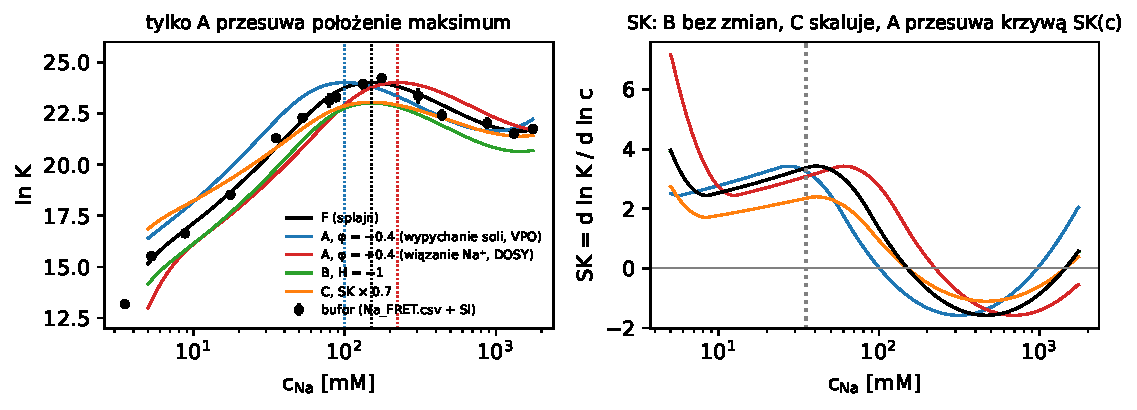
\includegraphics[width=0.9\linewidth]{predictions_ABC.pdf}
\caption{Przewidywania A, B, C na naszym $F$ (\texttt{Na\_FRET.csv} + punkty $>$175 mM z SI, splajn): tylko A przesuwa maksimum (kropkowane linie). Skrypt \texttt{predictions\_ABC.py}.}
\label{fig:abc}
\end{figure}

\section{Bielec et al. 2022: digitalizacja Fig.~S3 i analiza A/B}

\textbf{Digitalizacja} (\texttt{digitize\_bielec\_s3.py}): raster ze strony 5 SI (2206$\times$1182 px), kalibracja z wykrytych ticków (0--120 mM = 331--1526 px; dekada = 151 px), markery wykryte po kolorze z otwarciem morfologicznym 9$\times$9 px (usuwa słupki błędów i linię przerywaną). Niepewność odczytu: $\pm0.02$ dekady dla markerów wykrytych automatycznie, $\pm0.05$ dla częściowo zasłoniętych, $\pm0.10$ dla odczytanych ręcznie (Ficoll 10 i 50 mM, Dextran 40k 50 mM). Linia „No crowders” to \textbf{dopasowanie potęgowe}, nie dane; z digitalizacji nachylenie $Y=2.51$, zgodne z $Y=2.51$ w tekście pracy. Dane: \texttt{bielec\_s3\_points\_final.csv}.

\begin{figure}[h]
\centering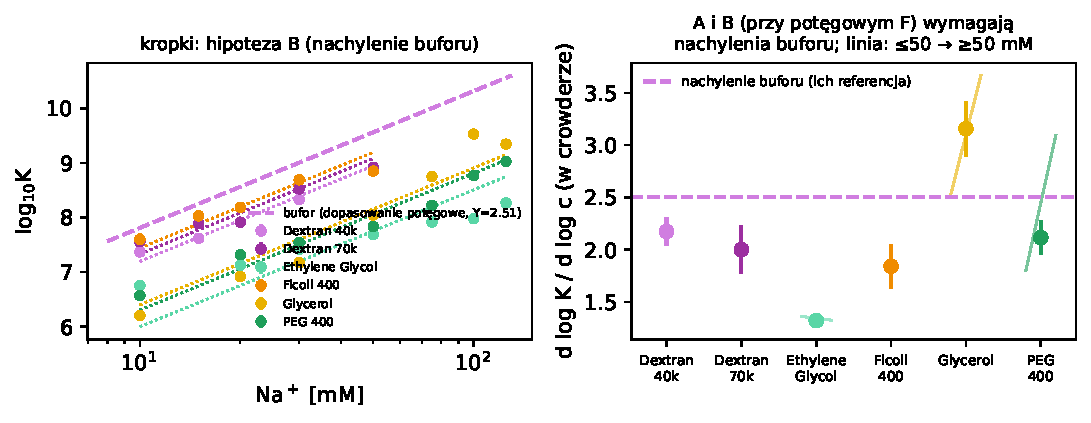
\includegraphics[width=0.95\linewidth]{ab_bielec_s3.pdf}
\caption{Lewo: Fig.~S3 zdigitalizowana; kropkowane linie to hipoteza B (nachylenie buforu, dopasowane przesunięcie $H$). Prawo: nachylenie $d\log K/d\log c$ w każdym crowderze vs nachylenie referencji buforowej (2.51); kreski: nachylenie $\le50$ i $\ge50$ mM. Skrypt \texttt{ab\_bielec\_s3.py}.}
\end{figure}

\begin{center}\small
\begin{tabular}{lccccccc}
\toprule
crowder (40 wt\%) & $n$ & mM & nachylenie & $\le$50 / $\ge$50 mM & $H$ [log] & rms B & $f_\text{zw}$ (A) przy $c_\text{min}\to c_\text{max}$\\
\midrule
EG & 7 & 10--125 & $1.32\pm0.06$ & 1.36 / 1.33 & $-1.81$ & 0.44 & 0.62 $\to$ 0.88\\
PEG 400 & 7 & 10--125 & $2.12\pm0.16$ & 1.80 / 3.09 & $-1.50$ & 0.20 & 0.68 $\to$ 0.76\\
glicerol & 7 & 10--125 & $3.16\pm0.27$ & 2.54 / 3.67 & $-1.41$ & 0.32 & 0.77 $\to$ 0.67\\
Dextran 40k & 4 & 10--50 & $2.17\pm0.13$ & -- & $-0.61$ & 0.10 & 0.33 $\to$ 0.48\\
Dextran 70k & 5 & 10--50 & $2.00\pm0.23$ & -- & $-0.48$ & 0.15 & 0.21 $\to$ 0.45\\
Ficoll 400 & 5 & 10--50 & $1.84\pm0.21$ & -- & $-0.37$ & 0.18 & 0.18 $\to$ 0.48\\
\bottomrule
\end{tabular}\end{center}
Uwagi: (a) Na referencji potęgowej czysty A i czysty B dają nachylenie 2.51; odchylenia (EG o 9 błędów standardowych) oznaczają $\partial S_K/\partial x\neq0$. (b) W modelu stałego $\kappa$ ($c_\text{wolny}=c/(1+\kappa c_\text{EO})$) ułamek związany $f_\text{zw}$ nie zależy od $c$, a z danych zależy, dla EG silnie. (c) Gdyby prawdziwe $F$ buforu było zakrzywione jak nasze ($S_K$ około 3.4 przy 35 mM, około 1.5 przy 125 mM), niskie nachylenie EG dałoby się formalnie uzyskać z A($\varphi<0$) tylko przy $\varphi\approx-1.5$ (aktywność $\times$4), a wtedy $K$ w EG byłoby \emph{wyższe} niż w buforze, a nie 100$\times$ niższe. EG to więc B (duże $H<0$) + C. (d) Fig.~S3 to pojedyncze miareczkowania z widocznym rozrzutem (glicerol: 100 mM powyżej 125 mM); wnioski dotyczą kierunku, nie trzeciego miejsca po przecinku. (e) Inna para znaczników (pojedynczy znacznik, metoda jasności) niż nasza para FRET.

\section{Literatura: szczegóły}
\textbf{Krótkie PEG i EG przy 0.1--1 M.} Nakano 2004 SI Tab. S1 \cit{b:nak04}\PT{} (8-mer, 25 °C): $\Delta\ln K$ przy 40\% PEG 200 wynosi $-5.1\pm1.3$ (0.12 M) i $-7.4\pm0.8$ (1.02 M). Czysty A wymagałby $\varphi=+6\ldots+30$, co jest niemożliwe, więc dominuje B. Ghosh 2023 \cit{b:gh23}\PT: $S_\text{sec}$ maleje monotonicznie z PEG 200 (kierunek przeciwny do A z $\varphi>0$; zgodny z A($\varphi<0$) przy $\mu_x>0$ albo z C). Autorzy jawnie zakładają addytywność (B) i testują ją tylko w skali $\Delta a_w$ \cit{b:gh20,b:gh23}.

\textbf{Długi PEG przy niskiej soli.} Markarian \& Schlenoff \cit{b:mark}\PT{} (zdigitalizowane Fig.~6 i 7A; nasze nachylenie 2.85 wobec 2.96 autorów): przy 30\% PEG $\Delta\ln K=+1.29$ (ln a = $-3.7$) i $-1.20$ ($-2.2$), przecięcie przy ln a $\approx-2.5\ldots-3.4$. Oś x to już aktywność z VPO, więc A „zdjęte”, a nachylenie i tak spada o 50\% na prawie prostym $F$: C. Nakano 2014 \cit{b:nak14}\PT{} (Fig.~3B zdigitalizowana; nachylenie buforu 1.82 vs 1.8 autorów): PEG 8000 $+0.77\to+0.32$ log K między 0.02 a 0.2 M (około $-4.6$~kJ/mol przy 20 mM, jak u nas). Autorzy proponują wprost człon $\varepsilon\times\log$[sól], czyli B + C. Karimata 2007 \cit{b:kar07}\ABS{}: ten sam obraz, liczby za paywallem.

\begin{figure}[h]
\centering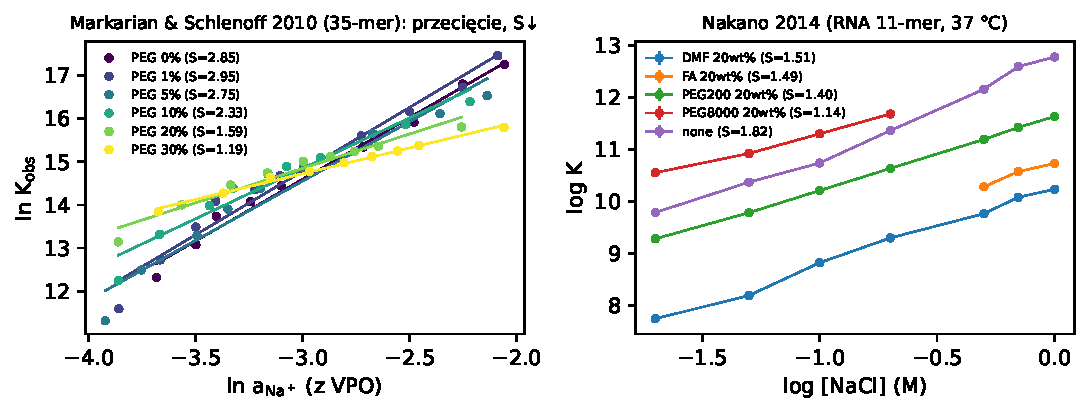
\includegraphics[width=0.95\linewidth]{lit_replot.pdf}
\caption{Dane zdigitalizowane w tym przeglądzie (\texttt{na\_markarian2010\_fig6.csv}, \texttt{na\_nakano2014\_fig3B.csv}; skrypt \texttt{lit\_replot.py}). Lewo: przy niskiej soli długi PEG stabilizuje, przy wyższej destabilizuje; nachylenie maleje z 2.85 do 1.19. Ani czysty A, ani czysty B tego nie dają. Prawo: PEG 8000 obniża nachylenie (1.14 vs 1.82 buforu w całym zakresie; 1.54 na tym samym odcinku 0.02--0.2 M), PEG 200 i DMF też, FA nie.}
\end{figure}

\textbf{Mg$^{2+}$ i RNA III-rzędowe.} „Crowder obniża potrzebne Mg$^{2+}$” to przesunięcie poziome, ale wszyscy autorzy przypisują je objętości wyłączonej. Hipotezę „PEG podnosi aktywność Mg$^{2+}$” sprawdzono przez VPO i odrzucono: Kilburn 2010 (przewidywane $c_m$ 0.675 vs obserwowane 0.21 mM) \cit{b:kil10}\PT, Desai 2014 (1.08$\to$0.79 mM; 0.91 w skali molalnej) \cit{b:desai}\PT. Kilburn 2013 \cit{b:kil13}\PT: współczynnik Hilla stały z PEG (Mg około 5.0, Na 1--1.5). Nasze przeliczenie: wspólne $\Delta\ln c_m$ dla Mg i Na (0.86 vs 0.93--1.40) wygląda jak A, autorzy wybrali objętość wyłączoną. Paudel 2014/2018: $K_\text{Mg}$ 11$\to$1.6 mM, 51$\to$20 mM \cit{b:pau14,b:pau18}\PT. Lambert \& Draper 2007: osmolity i Mg$^{2+}$ nieaddytywne, ze zmianą znaku przy wysokim Mg$^{2+}$ \cit{b:ld07}\PT.

\textbf{Białko--DNA (Record).} Hong 2005 \cit{b:hong05}\PT: mocznik $-1.7\pm0.2$~m$^{-1}$ wspólne dla 0.21 i 0.43 m K$^+$ ($\partial S/\partial x\approx0$); korekta aktywności z VPO $-0.34$ (mocznik), $-0.37$ (betaina), około 20\% efektu. Kontur 2006 i Vander Meulen 2008 stosują tę samą procedurę \cit{b:kontur,b:vdm}\PT.

\textbf{Teoria.} W ramie kondensacji Manninga $S_K\propto\Delta(1/\xi)$, $\xi\propto1/\varepsilon$, więc gdy obie formy są w reżimie kondensacji, $S_K\propto\varepsilon$ (nasze wyprowadzenie, prace źródłowe \cit{b:mann72,b:rec78} nieczytane w tym zadaniu). Dla Nakano 2014 PEG 8000 obserwowane 1.14/1.54 = 0.74. Spadek $S_K$ przez kosolut jest więc oczekiwany i nie wymaga zmiany aktywności soli.

\section{Co jest nowe w naszym podejściu i czym musi się różnić}
\begin{enumerate}[leftmargin=*]
\item \textbf{Maksimum $F$ jako dyskryminator.} Przesunięcie maksimum wzdłuż $\ln c$ jest sygnaturą wyłącznie A. B przesuwa w pionie, C skaluje wysokość, ale żadne nie przesuwa położenia. Tego testu w literaturze nie ma.
\item \textbf{Spójność ilościowa.} A z jedną funkcją $\varphi(x)$ musi jednocześnie dać $\Delta\ln K$ przy każdym $c$, przesunięcie $c_\text{max}$ i $\partial S_K/\partial x=-\varphi'F''$. Recenzent zacytuje Lambert/Leipply/Draper (C bez A) i Knowles (VPO PEG--KCl, $\varphi<0$), a niezależna miara $\varphi$ z VPO już istnieje dla soli naszego buforu (Na$_2$HPO$_4$, NaCl; Knowles 2015, $\varphi<0$). Własny pomiar VPO przy dokładnie naszym pH (z H$_2$PO$_4^-$) i 20 mM byłby tylko potwierdzeniem.
\item \textbf{Ograniczenia, które trzeba przewidzieć:} maksimum przy około 150 mM ma $K\approx3\cdot10^{10}$, czyli tuż przy suficie oznaczalności przy 10 nM donora; wysoka sól i PEG mogą rozwarstwiać się (PEG 8000 powyżej 0.2 M u Nakano); para FRET może zmieniać się z solą i crowderem (osobna kontrola z pojedynczym znacznikiem).
\end{enumerate}

\textbf{Przewidywania na naszym $F$} (\texttt{predictions\_ABC.json}; splajn przez 15 punktów buforu, maksimum przy 151 mM, $S_K(35\,\text{mM})=3.38$):
\begin{center}\small
\begin{tabular}{lccc}
\toprule
scenariusz & $c_\text{max}$ [mM] & $\ln K_\text{max}$ względem buforu & $S_K$ przy 35 mM\\
\midrule
bufor & 151 & 0 & 3.38\\
A, $\varphi=-0.4$ (wypychanie soli, kierunek z VPO) & 100 & 0 & 3.26\\
A, $\varphi=+0.4$ (wiązanie Na$^+$, kierunek z DOSY) & 224 & 0 & 3.08\\
B, $H=-1$ & 151 & $-1.0$ & 3.38\\
C, $S_K\times0.7$ (wokół 35 mM) & 151 & $-0.96$ & 2.36\\
\bottomrule
\end{tabular}\end{center}
Uwaga: przy 35 mM nasze $S_K$ jest blisko lokalnego maksimum, więc samo nachylenie przy 35 mM słabo rozróżnia A, a silnie C. Rozstrzyga położenie maksimum. Kształt splajnu przy $c<10$ mM jest niepewny (mało punktów) i nie wpływa na wnioski dla 35--600 mM.

\textbf{Proponowany projekt.} Bufor + EG 20, 40\% + PEG 400 40\% + PEG 35k 10\% (1 nM donora); Na$^+$: 10, 20, 35, 50, 75, 100, 150, 200, 300, 450, 600 mM (gęsto wokół maksimum). Dopasować globalnie $F$ (splajn) oraz dla każdego crowdera $\{\varphi,H,\lambda\}$ (A + B + C), porównać $\varphi$ z VPO ($\mu_x$). Kryterium: $|\Delta\ln c_\text{max}|\ge0.2$ przy niepewności $\le0.1$.

\section*{Bibliografia}
\small
\begin{enumerate}[label={[\arabic*]},ref={\arabic*},leftmargin=*,itemsep=0pt]
\item\label{b:nak04} Nakano S., Karimata H., Ohmichi T., Kawakami J., Sugimoto N. The Effect of Molecular Crowding with Nucleotide Length and Cosolute Structure on DNA Duplex Stability. \emph{J. Am. Chem. Soc.} 126, 14330 (2004). DOI 10.1021/ja0463029. [CR; PT+SI]
\item\label{b:gh20} Ghosh S., Takahashi S., Ohyama T., Endoh T., Tateishi-Karimata H., Sugimoto N. Nearest-neighbor parameters for predicting DNA duplex stability in diverse molecular crowding conditions. \emph{PNAS} 117, 14194 (2020). DOI 10.1073/pnas.1920886117. [CR; PT+SI]
\item\label{b:gh23} Ghosh S., Takahashi S., Banerjee D., et al., Sugimoto N. Nearest-neighbor parameters for the prediction of RNA duplex stability in diverse in vitro and cellular-like crowding conditions. \emph{Nucleic Acids Res.} 51, 4101 (2023). DOI 10.1093/nar/gkad020. [CR; PT+SI]
\item\label{b:nak14} Nakano S., Kitagawa Y., Miyoshi D., Sugimoto N. Hammerhead ribozyme activity and oligonucleotide duplex stability in mixed solutions of water and organic compounds. \emph{FEBS Open Bio} 4, 643 (2014). DOI 10.1016/j.fob.2014.06.009. [CR; PT]
\item\label{b:nak16} Nakano S., Tanino Y., Hirayama H., Sugimoto N. Thermal Stability of RNA Structures with Bulky Cations in Mixed Aqueous Solutions. \emph{Biophys. J.} 111, 1350 (2016). DOI 10.1016/j.bpj.2016.08.031. [CR; PT]
\item\label{b:mark} Markarian M.Z., Schlenoff J.B. Effect of Molecular Crowding and Ionic Strength on the Isothermal Hybridization of Oligonucleotides. \emph{J. Phys. Chem. B} 114, 10620 (2010). DOI 10.1021/jp103213w. [CR; PT]
\item\label{b:kar07} Karimata H., Nakano S., Sugimoto N. Effects of Polyethylene Glycol on DNA Duplex Stability at Different NaCl Concentrations. \emph{Bull. Chem. Soc. Jpn.} 80, 1987 (2007). DOI 10.1246/bcsj.80.1987. [CR; ABS]
\item\label{b:llld10} Lambert D., Leipply D., Draper D.E. The Osmolyte TMAO Stabilizes Native RNA Tertiary Structures in the Absence of Mg$^{2+}$: Evidence for a Large Barrier to Folding from Phosphate Dehydration. \emph{J. Mol. Biol.} 404, 138 (2010). DOI 10.1016/j.jmb.2010.09.043. [CR; PT]
\item\label{b:ld12} Lambert D., Draper D.E. Denaturation of RNA Secondary and Tertiary Structure by Urea: Simple Unfolded State Models and Free Energy Parameters Account for Measured m-Values. \emph{Biochemistry} 51, 9014 (2012). DOI 10.1021/bi301103j. [CR; PT]
\item\label{b:ld07} Lambert D., Draper D.E. Effects of Osmolytes on RNA Secondary and Tertiary Structure Stabilities and RNA-Mg$^{2+}$ Interactions. \emph{J. Mol. Biol.} 370, 993 (2007). DOI 10.1016/j.jmb.2007.03.080. [CR; PT]
\item\label{b:hong05} Hong J., Capp M.W., Saecker R.M., Record M.T. Jr. Use of Urea and Glycine Betaine To Quantify Coupled Folding and Probe the Burial of DNA Phosphates in Lac Repressor$-$Lac Operator Binding. \emph{Biochemistry} 44, 16896 (2005). DOI 10.1021/bi0515218. [CR; PT]
\item\label{b:kontur} Kontur W.S., Saecker R.M., Davis C.A., Capp M.W., Record M.T. Jr. Solute Probes of Conformational Changes in Open Complex (RPo) Formation by Escherichia coli RNA Polymerase at the $\lambda$PR Promoter\ldots \emph{Biochemistry} 45, 2161 (2006). DOI 10.1021/bi051835v. [CR; PT]
\item\label{b:vdm} Vander Meulen K.A., Saecker R.M., Record M.T. Jr. Formation of a Wrapped DNA--Protein Interface: Experimental Characterization and Analysis of the Large Contributions of Ions and Water to the Thermodynamics of Binding IHF to H$'$ DNA. \emph{J. Mol. Biol.} 377, 9 (2008). DOI 10.1016/j.jmb.2007.11.104. [CR; PT]
\item\label{b:kn11} Knowles D.B., LaCroix A.S., Deines N.F., Shkel I., Record M.T. Jr. Separation of preferential interaction and excluded volume effects on DNA duplex and hairpin stability. \emph{PNAS} 108, 12699 (2011). DOI 10.1073/pnas.1103382108. [CR; PT+SI]
\item\label{b:kil10} Kilburn D., Roh J.H., Guo L., Briber R.M., Woodson S.A. Molecular Crowding Stabilizes Folded RNA Structure by the Excluded Volume Effect. \emph{J. Am. Chem. Soc.} 132, 8690 (2010). DOI 10.1021/ja101500g. [CR; PT]
\item\label{b:kil13} Kilburn D., Roh J.H., Behrouzi R., Briber R.M., Woodson S.A. Crowders Perturb the Entropy of RNA Energy Landscapes to Favor Folding. \emph{J. Am. Chem. Soc.} 135, 10055 (2013). DOI 10.1021/ja4030098. [CR; PT]
\item\label{b:desai} Desai R., Kilburn D., Lee H.-T., Woodson S.A. Increased Ribozyme Activity in Crowded Solutions. \emph{J. Biol. Chem.} 289, 2972 (2014). DOI 10.1074/jbc.M113.527861. [CR; PT]
\item\label{b:pau14} Paudel B.P., Rueda D. Molecular Crowding Accelerates Ribozyme Docking and Catalysis. \emph{J. Am. Chem. Soc.} 136, 16700 (2014). DOI 10.1021/ja5073146. [CR; PT]
\item\label{b:pau18} Paudel B.P., Fiorini E., Börner R., Sigel R.K.O., Rueda D.S. Optimal molecular crowding accelerates group II intron folding and maximizes catalysis. \emph{PNAS} 115, 11917 (2018). DOI 10.1073/pnas.1806685115. [CR; PT]
\item\label{b:mann72} Manning G.S. On the application of polyelectrolyte ``limiting laws'' to the helix-coil transition of DNA. I. Excess univalent cations. \emph{Biopolymers} 11, 937 (1972). DOI 10.1002/bip.1972.360110502. [CR; nieczytane]
\item\label{b:rec78} Record M.T. Jr., Anderson C.F., Lohman T.M. Thermodynamic analysis of ion effects on the binding and conformational equilibria of proteins and nucleic acids\ldots \emph{Q. Rev. Biophys.} 11, 103 (1978). DOI 10.1017/s003358350000202x. [CR; nieczytane]
\item\label{b:bielec22} Bielec K., Kowalski A., Bubak G., Witkowska Nery E., Hołyst R. Ion Complexation Explains Orders of Magnitude Changes in the Equilibrium Constant of Biochemical Reactions in Buffers Crowded by Nonionic Compounds. \emph{J. Phys. Chem. Lett.} 13, 112 (2022). DOI 10.1021/acs.jpclett.1c03596. [CR; PT+SI]
\end{enumerate}
Pełne listy (ok. 80 pozycji) z oznaczeniem dostępu: \texttt{na\_notes.md}, \texttt{mg\_notes.md}; weryfikacja Crossref: \texttt{na\_crossref\_check.txt}, \texttt{mg\_crossref\_check.txt}.
\end{document}
